% Print
\documentclass[DIV=15,headinclude=true]{scrartcl}

%Packages, die für die deutsche Sprache erforderlich sind
\usepackage[utf8]{inputenc}
\usepackage[T1]{fontenc}
\usepackage{lmodern}
\usepackage[ngerman]{babel}
\usepackage{csquotes}

%Packages für Graphik
\usepackage[]{graphicx}
\graphicspath{{figures/}}

%BibLaTex
\usepackage[backend=biber]{biblatex}
\addbibresource{literature/bibliography.bib} 

%Package, damit Bibtex-URL klappt
\usepackage[pdfusetitle]{hyperref}
\usepackage{url}

%Noch schönere Typographie
\usepackage{microtype}

%Kästen
\usepackage{framed}

%%%%% BEGINN KOPF- UND FUẞZEILE %%%%%
\usepackage[headsepline,footsepline]{scrlayer-scrpage}
\usepackage{graphicx}
\pagestyle{scrheadings}
\ohead{\includegraphics[height=1cm]{figures/bluemarble}}
\chead{\headmark}
\automark{section}
%\ihead{\includegraphics[height=1cm]{bluemarble.jpg}}
\ifoot{\csname @title\endcsname}\cfoot{\pagemark}
\ofoot{\today}
%%%%% ENDE KOPF- UND FUẞZEILE %%%%%

\begin{document}
%%%%% BEGINN TITEL %%%%%
\title{Projektaufgabe}
\subtitle{Entwicklungsmethoden Nachhaltiger Produkte}
\author{EnWiNaP-Team}
\maketitle
%%%%% ENDE TITEL %%%%%

%%%%% BEGINN FRONT MATTER %%%%%
\tableofcontents
%%%%% ENDE FRONT MATTER %%%%%


%%%%% BEGINN INHALT %%%%%
\begin{framed}

	Als grobe Richtlinie für den Umfang der Arbeit könnt ihr
	\textasciitilde30 Seiten annehmen. Im Allgemeinen gilt jedoch: Kürzer
	ist (so lange alle Aufgaben bearbeitet sind) besser!

\end{framed}

\section{Hintergrund}

Smartphones sind für die überwiegende Mehrheit der Menschen in
Deutschland ein fester Bestandteil des Alltags und des
Selbstverständnisses geworden. Sie werden für die Arbeit, für die
Informationsbeschaffung, zum Einkaufen und natürlich für die Gewinnung
von und Interaktion mit sozialen Kontakten genutzt. Der Psychologe
Christian Montag beschreibt dies als ``ausgelagertes Gehirn'', welches
des Menschen Vorteile dabei verschafft, ihren Alltag zu meistern
\cite{Spanke2019}. Gleichzeitig sieht er aber auch, dass sich ein
Suchtverhalten und Konditionierungsmechanismen einstellen, die die
Menschen dazu bringen, immer mehr Zeit mit diesen Geräten zu verbringen
und ihnen einen hohen Stellenwert in ihrem Leben einzuräumen. Das
erklärt auch, dass in Deutschland im Jahr 2019 rund 22 Millionen
Smartphones verkauft wurden \cite{Tenzer2020}; weltweit waren es in
diesem Zeitraum über 1,3 Milliarden Geräte \cite{Tenzer2020a}. Obwohl
die Verkaufszahlen in den letzten Jahren leicht rückläufig sind, sind
dies immer noch beeindruckende Mengen an technischen Geräten. Technische
Geräte, die kritische Ressourcen benötigen welche kaum recycelt werden,
für hohe Schadstoffemissionen sowie für einen hohen Wasser- und
Energieverbrauch verantwortlich sind, immer wieder mit ausbeuterischen
und gefährlichen Arbeitsbedingungen in Verbindung gebracht werden und im
Schnitt lediglich 33 Monate genutzt werden \cite{Jardim2017, Odea2020}.

Es stellt sich die Frage, ob in einer Gesellschaft, die immer mehr nach
nachhaltigen Produkten verlangt, dieses Verständnis des Smartphones noch
zeitgemäß ist. Und tatsächlich beweisen kleine Firmen wie Fairphone
(\url{https://www.fairphone.com/de/}) oder Shift
(\url{https://www.shiftphones.com/}), dass es bereits einen (wenn auch
kleinen) Markt für Smartphones gibt, die eine höhere Nachhaltigkeit
versprechen.

Aber lässt sich so wirklich etwas verändern? Gibt es Rebound-Effekte
oder ist das Ganze vielleicht sogar nur ``Greenwashing''? Könnte ein
umgedachtes Produkt den (schädlichen) Umgang der Nutzer\_innen
verändern? Und ließe sich mit einem wirklich nachhaltigeren Smartphone
ein Business Case aufmachen?

\subsection{Fallstudie}

Die oben gestellten Fragen haben euch dazu bewegt, aktiv zu werden. Als
junge Ingenieur\_innen seht ihr hier eine Herausforderung, der ihr euch
gerne stellen möchtet. Wäre es nicht eine Möglichkeit, als Startup
Smartphones komplett neu zu denken um den Kunden ein faires,
nachhaltigeres und langlebigeres Produkt anbieten zu können?

Als ersten Schritt wollt ihr mit diesem Bericht eine grundsätzliche
Analyse des Sachverhaltes liefern. Er soll den ist-Zustand des Produktes
beleuchten und mithilfe bestehender Studien dessen Probleme
herausarbeiten. Außerdem soll eine Abschätzung der Potentiale für ein
verbessertes Produkt erfolgen. Dabei sollen Überlegungen zu den Werten
der Technologie, relevanten Stakeholdern, geeigneten Konstruktions- und
Entwicklungsmethoden sowie den Arbeitsbedingungen einfließen. Außerdem
soll der Ansatz für eine Lebenszyklusanalyse aufgestellt werden, um die
sozialen, monetären und ökologischen Auswirkungen der neuen Produktidee
quantifizieren zu können. Zusammenfassend wollt ihr mit diesem Bericht
folgende übergeordnete Fragestellung beantworten:

\emph{Kann ein kleines in Deutschland ansässiges Unternehmen die
	Nachhaltigkeit eines Smartphones in allen Dimensionen signifikant
	steigern?}

\section{Technik \& Werte}

\begin{enumerate}
	\item
	      Welche Techniken und Technologien verwendet das Produkt aus der
	      Projektaufgabe? Wie können sie kategorisiert werden? (Empfehlung:
	      Mindmap o. Ä. für eine mögliche Kategorisierung, andere kurz
	      erläutern)
	\item
	      Beschreibt, warum das Produkt der Projektaufgabe als
	      ``Organerweiterung'' oder ``Gehirnerweiterung'' betrachtet werden
	      kann, um Mängel des Menschen auszugleichen, und warum als Ausdruck des
	      ``Machbaren'', als Selbstzweck, dem die Kultur- und Wertvorstellungen
	      untergeordnet wurden. Welche Beschreibung macht mehr Sinn? Sind alle
	      Gruppenmitglieder derselben Meinung? Wenn nicht, verfasst zwei
	      Absätze, die beide Meinungen darstellen.
\end{enumerate}

\section{Technikbewertung} \label{technikbewertung}

\begin{enumerate}
	\item
	      VDI 3780

	      \begin{enumerate}
		      \item
		            Was sind Werte, die im Kontext des Produktes stehen? Welche sind
		            individuelle Bedürfnisse, welche gesellschaftliche Präferenzen oder
		            Notwendigkeiten?
		      \item
		            In welchem Verhältnis stehen diese Werte zueinander? (Empfehlung:
		            Diagramm wie VDI 3780 Bild 3)
		      \item
		            Was sind typische Entwicklungsziele für das Produkt der
		            Projektaufgabe (Ist- und Sollzustand)? \label{entwicklungsziele}
		      \item
		            Wie stehen die Entwicklungsziele im Zusammenhang mit den Werten?
		            Erstelle ein Diagramm/Abbildung, das die Hierarchie und
		            Interaktionen der Werte und Ziele vereinigt.
	      \end{enumerate}
	\item
	      Vorsorgeprinzip/Nachsorgeprinzip

	      \begin{enumerate}
		      \item
		            Wo am betrachteten Produkt wurde bereits das Vorsorgeprinzip
		            angewendet?
		      \item
		            Wo wurde bisher das Vorsorgeprinzip nicht angewendet? Ist es
		            gescheitert?
	      \end{enumerate}
\end{enumerate}

\section{Anforderungsanalyse}

Wie kommen wir von den Entwicklungszielen (Abschnitt \ref{technikbewertung} Aufgabe
\ref{entwicklungsziele}) zu den Anforderungen?

\begin{enumerate}
	\item
	      Aufstellen der Anforderungen in Form einer Anforderungsliste.

	      \begin{enumerate}
		      \item
		            Wer sind typische Stakeholder für das Produkt der Projektaufgabe?
		            Identifiziert diese und ordnet diese den verschiedenen
		            Entwicklungszielen zu. Diskutiert auch den Fokus der Stakeholder.
		      \item
		            Welche Anforderungen können diese Stakeholder an das Produkt der
		            Projektaufgabe haben? Wie lassen sich Konflikte zwischen den
		            Anforderungen lösen? Verwendet dafür die übergeordneten Werte aus
		            Technikbewertung. Sammelt eure Gedanken in Form eines Brainstormings
		            und bildet Cluster für die Stakeholder.
	      \end{enumerate}
\end{enumerate}

\section{Energie und Material}

\subsection{Lebenszykluskosten (Life Cycle Costing)}

Zu dem Thema "`Computer System Life Cycle Costing"' wird euch
\href{https://tubcloud.tu-berlin.de/s/nLs4njSqBxrXLS3}{hier}\footnote{\texttt{https://tubcloud.tu-berlin.de/s/nLs4njSqBxrXLS3}}
eine Forschungsarbeit zur Verfügung gestellt. Beantwortet bitte die
folgenden Fragen:

\begin{enumerate}
	\item
	      Schreibt einen Bericht über die Lebenszykluskosten von
	      Computersystemen
	\item
	      Nehmen wir an, dass die Anschaffungskosten (Acquisition Cost) und die
	      erwartete Nutzungsdauer eines Computersystems 500 € bzw. 3 Jahre
	      betragen. Die erwartete Anzahl der Ausfälle des Computersystems pro 1
	      Millionen Stunden liegt bei 80, und die einzigen Betriebskosten des
	      Systems sind die Kosten der korrektiven Wartung (Maintenance Cost).
	      Rechnet die Lebenszykluskosten eines Computersystems aus, wenn die
	      Kosten für jeden korrektiven Wartungseinsatz 150 € und der jährliche
	      Rabatt oder Zinssatz 6\% betragen.
	\item
	      Erläutert die größten Schwierigkeiten bei der Schätzung der
	      Softwarekosten
	\item
	      Erläutert die Faktoren, die die Software-Lebenszykluskosten
	      beeinflussen
	\item
	      Was ist der Unterschied zwischen den Kosten für Computerhardware und
	      -software?
	\item
	      Erläutert Methoden der Software-Kostenschätzung
\end{enumerate}

\subsection{Material Flow Analysis}

In den Anhängen befinden sich zwei Forschungsarbeiten:

\begin{enumerate}
	\item
	      Material Flow Analysis and Energy Requirements of Mobile Phone
	      Material Recovery Processes
	      (\href{https://tubcloud.tu-berlin.de/s/TPze3EZKfX9EEaf}{Link}\footnote{\texttt{https://tubcloud.tu-berlin.de/s/TPze3EZKfX9EEaf}})
	\item
	      Quantitative Analysis of Material Flow of Used Mobile Phones in Japan
	      (\href{https://tubcloud.tu-berlin.de/s/fEJRArZMbxyQeX8}{Link}\footnote{\texttt{https://tubcloud.tu-berlin.de/s/fEJRArZMbxyQeX8}})
\end{enumerate}

Bitte beantwortet nach dem Lesen und Analysieren der Papiere die
folgenden Fragen:

\begin{enumerate}
	\item
	      Welche Komponenten wurden in der Materialflussanalyse für die
	      Mobiltelefone als die folgenden betrachtet

	      \begin{enumerate}
		      \item
		            Stoffe (Substances)
		      \item
		            Waren (Goods)
		      \item
		            Aktivität (Activity)
		      \item
		            Fluss und Strömung (Flow \& Flux)
	      \end{enumerate}
	\item
	      Was wurde als System definiert und was sind die Systemgrenzen?
	\item
	      Wie ist die Auswahl der Substanzen eurer Meinung nach durchgeführt
	      worden?
	\item
	      Welche Rolle spielt die Energie, um Mobiltelefone nachhaltig zu
	      machen?

	      \begin{enumerate}
		      \item
		            Wie wird das Recycling oder die Rückgewinnung der Telefone auf der
		            Basis von Energie- und Materialfluss nachhaltig gestaltet?
		      \item
		            Schlagt Schritte oder Methoden vor, die ihr im Hinblick auf die
		            Durchführung einer Materialflussanalyse für das Mobiltelefon anders
		            durchgeführt hättet.
	      \end{enumerate}
\end{enumerate}

\subsection{Ökobilanz und Social Life Cycle Assessmentn eines Smartphones}

Erstellung einer Ökobilanz sowie eines Social LCAs

\begin{enumerate}
	\item
	      Recherchiert bereits durchgeführte Studien zu Smartphones

	      \begin{enumerate}
		      \item
		            Vergleicht diese bezüglich folgender Punkte: Ziel und
		            Untersuchungsrahmen, Daten der Sachbilanzphase, Wirkungskategorien
		            der Wirkungsabschätzung, Ergebnisse
		      \item
		            Wer hat die Studie durchgeführt? An wen ist die Studie adressiert?
		            Spielen die von euch definierten Stakeholder eine Rolle
		            (Anforderungsanalyse 1.a)? Wenn ja, welche? Wenn nein, wieso werden
		            diese hier nicht angesprochen?
		      \item
		            Zieht ein Fazit: Was wird in den Studien gut und ausreichend
		            abgebildet, wo seht ihr Mängel? Was würdet ihr an den Studien wie
		            verändern?
	      \end{enumerate}
	\item
	      Erarbeitet Ziel und Untersuchungsrahmen für eine eigene Ökobilanz bzw.
	      ein eigenes social life cycle assessment eines Smartphones mit Hilfe
	      der DIN EN ISO 14040 und DIN EN ISO 14044
	\item
	      Erarbeitet eine Aufstellung der benötigten Daten für eine Sachbilanz:
	      Materialien, Energie, Stakeholdergruppen, mögliche EoL-Wege (Hier
	      sollt ihr nicht Daten suchen, sondern bestimmen, welche Daten benötigt
	      werden)
	\item
	      Freiwillige Zusatzaufgabe/Ersatzaufgabe für Aufgabe 1a-c (ggf.
	      Mehraufwand) - Eigenes Arbeiten mit OpenLCA und Ecoinvent (Datenbank
	      kann vom Fachgebiet bereitgestellt werden): Baut mit Hilfe der
	      Datenbank Ecoinvent eine Ökobilanz für ein Smartphone auf (mit Hilfe
	      von Aufgabenteil 2 und 3); führt eine Wirkungsabschätzung sowie eine
	      Auswertung durch und dokumentiert die Durchführung und die Ergebnisse
\end{enumerate}

\section{Arbeitswelt}

\begin{enumerate}
	\item
	      Aufstellen eines Produktionsprozesses (gesamte Wertschöpfungskette)
	      für das Produkt.
	\item
	      Ziehen einer geeigneten Systemgrenze (wie weit kann euer (kleines)
	      unternehmen die Kette beeinflussen)
	\item
	      Untersuchung der Produktionsschritte innerhalb der Systemgrenze.
	      Festlegung der Art des Produktionsschritts (manuell /
	      teilautomatisiert / automatisiert)
	\item
	      Festlegung der Bedingungen der manuellen Arbeit. Dazu gehört, wo die
	      Arbeit ausgeführt wird, welche Arbeitsatmosphäre angestrebt wird, wie
	      viel Lohn gezahlt wird, wie viele Tage gearbeitet wird.
	\item
	      Erörterung der Vor- und Nachteile der gewählten Arbeitsbedingungen in
	      Bezug auf die ProduzentInnen, die Qualität des Produktes, die Kosten
\end{enumerate}

\section{Konstruktionsmethoden}

\begin{enumerate}
	\item
	      \textbf{Bewertung}. Den Umwelteinfluss des Produktes (wie es heute
	      ist) und seines Herstellungsprozesses bewerten.

	      \begin{enumerate}
		      \item
		            Eine von den präsentierten Methoden auswählen und für die
		            Produktbewertung benutzen. \textbf{Wichtig}: \underline{begründen}
		            warum das spezifische Tool ausgewählt wurde.
		      \item
		            Anhand der ausgewählten Methode, die Umweltrelevantesten Aspekten
		            des Produktes identifizieren. Welche Teile / Herstellungsprozessen /
		            Materialen haben den größten (negativen) Einfluss auf die Umwelt? Wo
		            gibt es Verbesserungspotential?\\
		            ~\\
		            \underline{Freiwillige Zusatzaufgabe:} eine zusätzliche Methode
		            auswählen (Auswahl begründen) und die Bewertung wiederholen. Wie
		            ähnlich sind die Ergebnisse? Werden neue wichtige Aspekte gezeigt?
		      \item
		            Den Umweltrelevantesten Aspekt für Schritt 2 (Re-Design) auswählen.
		            Auswahl \underline{begründen}!
	      \end{enumerate}
	\item
	      \textbf{Re-Design}. Die Ergebnisse von Schritt 1 weitererentwickeln,
	      um das Produkt nachhaltiger zu gestalten.

	      \begin{enumerate}
		      \item
		            Eine Eco-Design Strategie auswählen. Wo soll der Fokus liegen --
		            z.B. Recycling / Abbau / Repair usw\ldots{}
		      \item
		            Verbesserungskonzepten brainstormen.
		      \item
		            Eine von den präsentierten Methoden auswählen und für die
		            Konzeptbewertung benutzen. \textbf{Wichtig}: \underline{begründen}
		            warum das spezifische Tool ausgewählt wurde.\\
		            ~\\
		            \underline{Freiwillige Zusatzaufgabe:} eine zusätzliche Methode
		            auswählen (Auswahl begründen) und die Bewertung wiederholen. Wie
		            ähnlich sind die Ergebnisse? Werden neue wichtige Aspekte gezeigt?
		      \item
		            Anhand der ausgewählten Methode, die Konzepte vergleichen und das
		            beste Konzept auswählen.
	      \end{enumerate}
\end{enumerate}
%%%%% ENDE INHALT %%%%%

%%%%% BEGINN BACK MATTER %%%%%
\cleardoublepage
\pagenumbering{Roman}
%Bibliographie
\printbibliography
%%%%% ENHDE BACK MATTER %%%%%
\end{document}
